\section{Design and Implementation}
\label{sec-design}
Our goal is to build a file system for a tiered storage hierarchy consisting of disks and NVM that combines the low latency of NVM and low cost of disk-based storage without regressing on performance while offering similar consistency guarantees as BPFS. This seems like a reasonable goal, however, it raises the some non-trivial questions about the overall design of such a tiered filesystem:

\begin{itemize}
\item How do we make changes to BPFS data structures so that it is able to locate the data in-memory or disk? \vspace{-0.1in}
\item What policies determine when to move data? \vspace{-0.1in}
\item Do we handle the disks directly or do we go through another file system to store data on disk? \vspace{-0.1in}
\item What is the ideal granularity at which we should move the data? \vspace{-0.1in}
\end{itemize}

We provide answers to these questions in this section and discuss at length, the policies and mechanisms required to implement the same. Figure~\ref{fig-bpfs} depicts the overall design of our system. We use NVM to store the filesystem metadata and all the filesystem operations are always done within the NVM tier. To preserve the filesystem consistency guarantees, we have opted for a simple design policy where only the data blocks are moved to the disks, while the metadata blocks always reside in the persistent NVM. Such a policy entails that for a given BPFS file, its data may be split across NVM and the disk. However, it is to be noted that even though a data block may be moved between the NVM and the disk, there will always be a single valid copy of that data block- whether in the disk or in the NVM.

The mechanism to determine the exact location of the valid copy of a given data block is through the use of the most significant bit(MSB) of the indirect pointer, pointing to the data block in the BPFS tree structure. This is also being depicted in the Figure~\ref{fig-bpfs}. If the MSB is not set, then the rest of the 63-bits denote a memory address of the data block within the NVM itself. While on the other hand, if the MSB is set, then the rest of the 63-bits denote a disk address where the data block was moved to on the disk. This answers the first question that we had raised earlier. In the following subsections, we discuss the design and implementation of Anti-Cache Manager and the Disk Manager that provide answers to the other design questions.

\subsection{Anti-Cache Manager}
In our design, NVM is the primary data store where all filesystem operations are being performed and hence, it contains the more frequently accessed blocks. We refer to such data residing in NVM as the `hot' data. Since the capacity of the persistent NVM is limited, we have to periodically evict blocks from NVM to disk, so that we can make space for more `hot' data. The evicted data on the disk is referred to as the `cold' data. While it is true that some of the `hot' data may become `cold' over time, it is also possible that some `cold' data will suddenly become `hot' and it has to be brought back in NVM. This is what we term as the `anti-caching' phenomenon- this gameplay between the `hot' and the `cold' data having a reverse caching effect. This anti-caching is at the heart of our implementation that enables us to amortize the cost of read-write operations equivalent to those provided by BPFS. We implement the well-known LRU-1 policy to distinguish the `hot' data blocks from the `cold' data blocks. We maintain a linked list of all the data block references. Whenever a data block is accessed, it is moved to the front of the linked list. Over time, the tail of the list will contain block references which have been least frequently accessed, while the head of the list will point to data blocks being most frequently accessed.

\begin{figure}
\centering
\vspace{-0.2in}
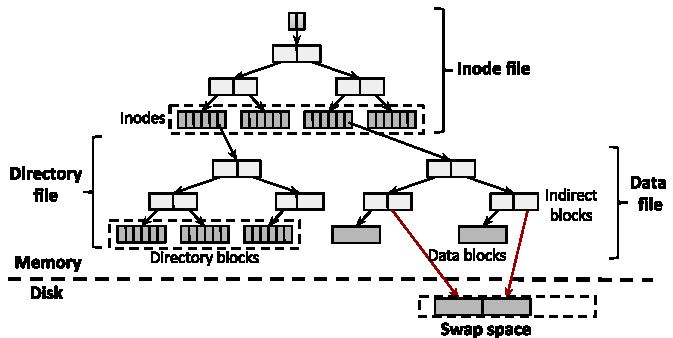
\includegraphics[width=0.5\textwidth]{figs/bpfs2.pdf}
\vspace{-0.2in}
\mycaption{fig-bpfstree}{BPFS tree structure}{\footnotesize The figure shows the file system organization of BPFS, along with our proposed modifications.}
\end{figure}

The Anti-Cache Manager component of the AC-BPFS filesystem implements the above proposed design policies. It runs as a separate background thread that continuously receives from the main AC-BPFS thread a stream of NVM data block references, in the order they are being accessed. It maintains an LRU data structure within itself and uses the LRU to evict a number of blocks according to the policy explained above. A soft threshold count of data blocks, known as `anti-caching threshold', is used to determine when and how many blocks to evict. The Anti-Cache Manager is made to poll arbitrarily every 10 ms on the size of the LRU list. If the size of the LRU list exceeds the specified anti-caching threshold of data blocks count in NVM, those many extra data blocks over the threshold are evicted from the tail of the list. This anti-caching threshold is set based on the latency of NVM writes and the polling time. We found that setting the anti-caching threshold to 80\% of the NVM size for a 10 ms polling duration is a good estimate. In order to ensure that data blocks that are currently being evicted to disk do not get updated by the file system, a block level locking mechanism is used which implicitly prevents any updates to the block.

\begin{figure}
\centering
\vspace{-0.2in}
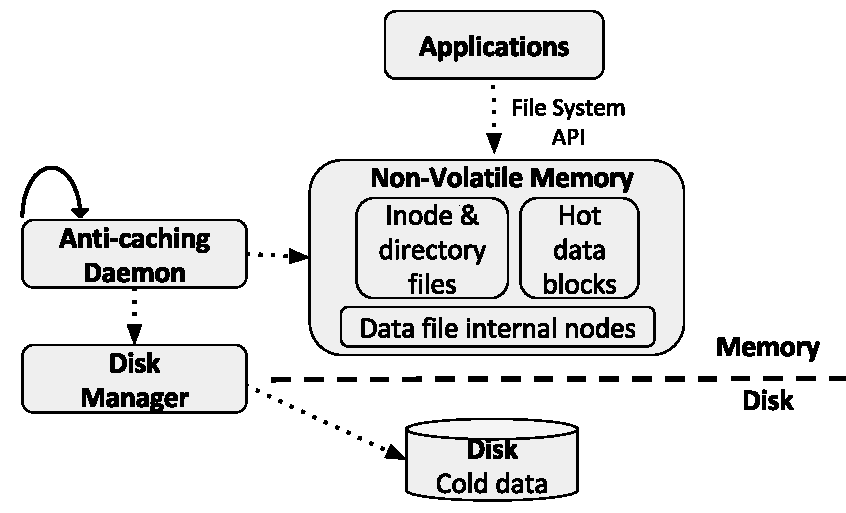
\includegraphics[width=0.5\textwidth]{figs/bpfs.pdf}
\vspace{-0.2in}
\mycaption{fig-bpfs}{Design Architecture of AC-BPFS}{\footnotesize The figure shows the overall design of our system.}
\end{figure}

This subsection answered our second question on the policies required to move data between NVM and the disk. The next subsection gives the answers to the remaining two questions.

\subsection{Disk Manager}
The Disk Manager component simulates a virtual disk using a file stored on disk in the BPFS partition of a predetermined size. It exposes APIs for reading and writing blocks into the disk individually and in bulk. It performs prefetching of additional blocks when a read is performed. The lifetime of the prefetched blocks in memory is predetermined to ensure that unused prefetched blocks are cleaned up regularly with the help of a background thread. To avoid fragmentation, a free list of blocks that have been freed is maintained. Since the disk manager writes blocks to a file, the buffer cache is used to buffer writes until all the blocks are written into the file. Our current implementation provides consistency at the expense of performance by notifying BPFS after persisting the blocks, which inturn updates the indirect pointer in the inodes to point to the new blocks through a blocking call.

The disk manager also exposes another write API to the Anti-Cache Manager to facilitate writing one block at a time, for faster random writes since any free block on disk can be used for writing and does not require sequential locality. To further improve performance in the case of bulk eviction of blocks from the anti-cache manager, the disk manager performs an explicit flush only after writing all the blocks on to the disk.

\subsection{File System Operations}
In this section we describe the workflows for various file system operations.
\subsubsection{Read}
When a read operation is performed on a file, the BPFS crawls the inode tree to the indirect block containing the pointer to the data block, identifies the location of the data block using the MSB that indicates whether the block is on disk or in NVM, then fetches the block into memory and asynchronously writes it back into NVM. Once the block is persisted in NVM, it frees the block on disk and updates the indirect pointer in the inode tree to point to the new block location in NVM atomically.

When a read operation is performed on a directory, the BPFS crawls the inode tree and the directory file blocks are loaded into memory from NVM and the necessary updates are made into the directory entry cache. It then traverses all the necessary inodes in the directory file and reads them from NVM.

\subsubsection{Write}
When a write operation is performed on a file, the BPFS traverses the inode tree to find the indirect block containing the pointers to the data block of the file and identifies the location of the data blocks. If the data block is in NVM, the write operation is performed in-place and has no additional overhead. If the data block is on disk, the block is fetched into NVM thus performing a copy on write of the data block and this block is updated and written back to NVM. The block on disk is then freed and the control comes back to the BPFS crawler. The indirect pointer in the inode tree is then updated to point to this new block location in-place along with in-place writes of the other internal nodes. The inode access time is also updated through an in-place atomic write.

\subsubsection{Open}
When a file is opened, the directory inode tree is parsed to find the file. If the file is not found and a create is requested, a new inode number is generated and the new inode is written to the inode file. Then the directory file is then updated. All these updates are performed in place. Since the metadata updates are in-place and in NVM, they are faster than usual disk writes and the additional overhead of metadata journaling can also be avoided by avoiding disk writes.
